\documentclass{article}
\usepackage{graphicx} % Required for inserting images
\usepackage[czech]{babel} % Nastaví češtinu
\addto\captionsczech{\renewcommand{\figurename}{Obr.}} % Změní "Obrázek" na "Obr."

\usepackage{hyperref}
\hypersetup{
    colorlinks=true,
    linkcolor=blue,
    filecolor=magenta,      
    urlcolor=blue,
}

\title{Jak na vektorizaci dálnic v N4CE}
\author{Mykhailo Radchenko}
\date{Březen 2026}

\begin{document}

\maketitle

\section{Příprava projektu}
Po spuštění softwaru N4CE začneme vytvořením nového datového prostředí. V panelu správy projektu klikneme pravým tlačítkem myši na položku \textbf{Models}, zvolíme možnost \textbf{New Normal}:
\begin{figure}[h]
    \centering
    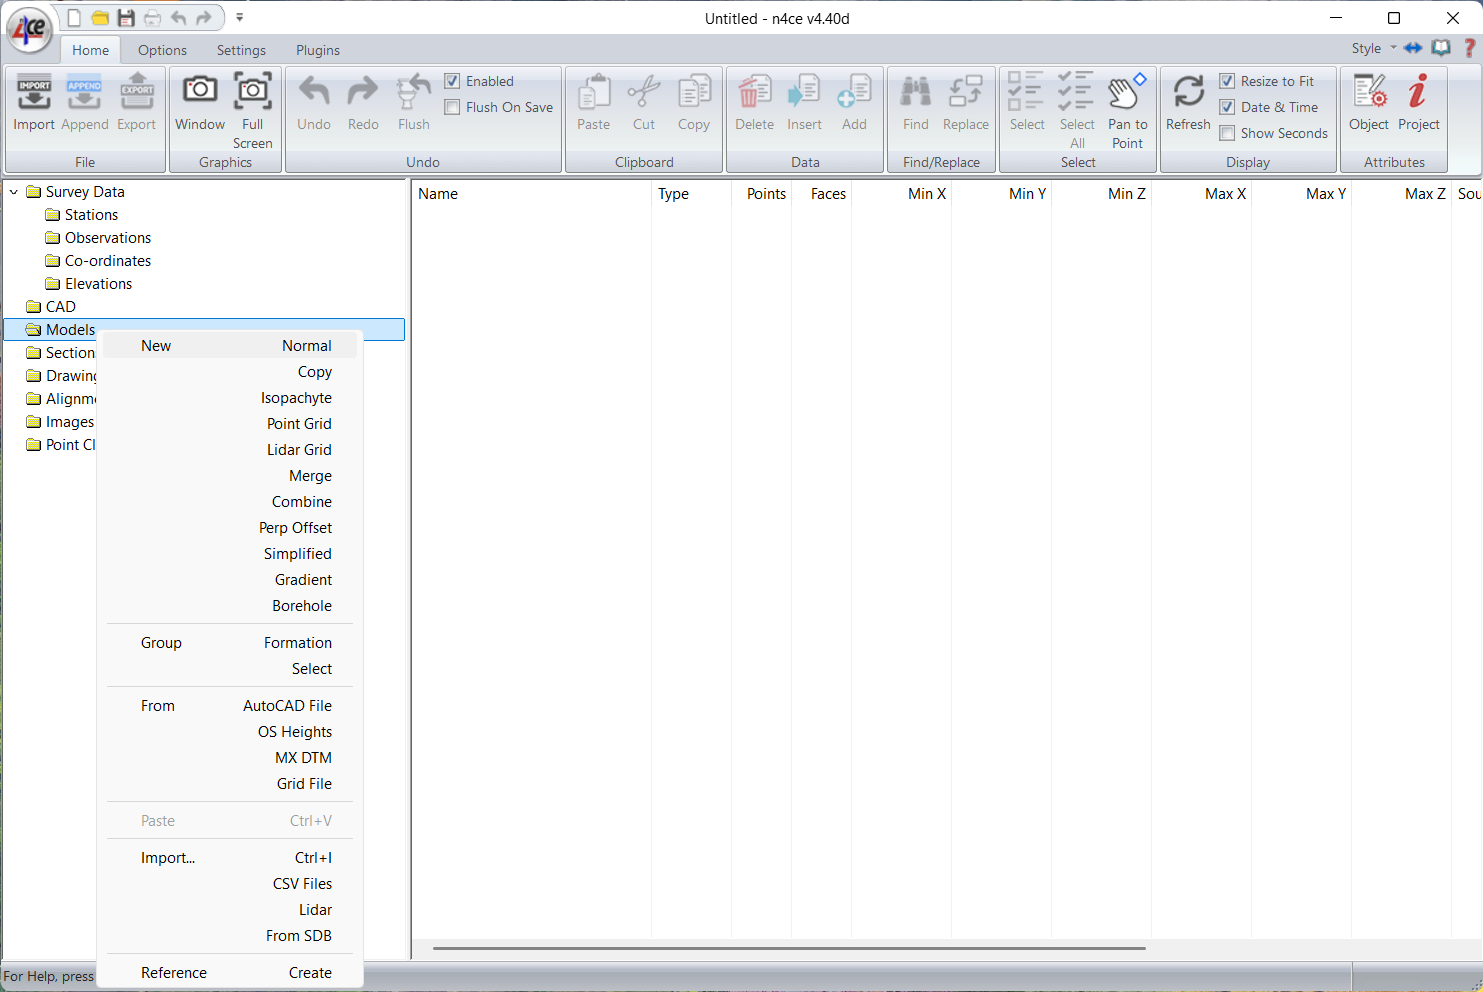
\includegraphics[width=1\linewidth]{obr1.png}
    \caption{Založení nového modelu typu Normal v prostředí N4CE}
\end{figure}
\newpage
Nový model smysluplně pojmenujeme (např. \textit{D1\_vektorizace}):
\begin{figure}[h]
    \centering
    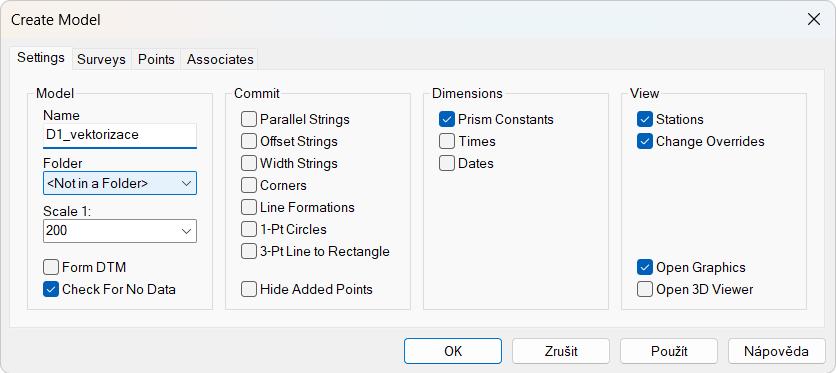
\includegraphics[width=1\linewidth]{obr2.png}
    \caption{Pojmenování nového modelu}
\end{figure}

Následně se zobrazí systémové upozornění \textit{„No data selected! Create a new model?“}, které potvrdíme volbou \textbf{Ano}. Následně se zobrazí okno „Layer Override“, které můžeme zavřít.

Otevře se nám pracovní okno modelu. Pro práci s prostorovými daty je následně nutné v horním pásu karet na záložce \textbf{Home} aktivovat režim \textbf{3D}, který nám zpřístupní nástroje pro manipulaci s mračnem bodů:
\begin{figure}[h]
    \centering
    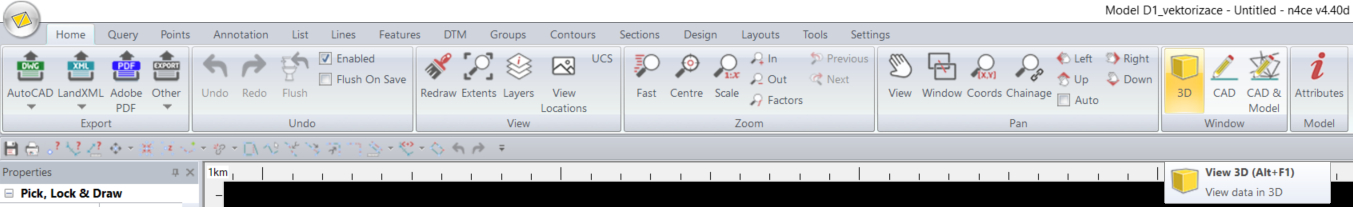
\includegraphics[width=1\linewidth]{obr3.png}
    \caption{Přepnutí do 3D pracovního prostředí na kartě Home}
\end{figure}

\section{Import dat}
Pro vektorizaci dálničního tělesa je potřeba korektně načíst mračna bodů a související panoramatické snímky z mobilního skenování. 

\subsection{Import mračen bodů} 
\begin{enumerate}
    \item V okně 3D zobrazení přejdeme na záložku \textbf{Point Cloud I/O} a zvolíme funkci \textbf{Convert to Octree}.
    \begin{figure}[h]
        \centering
        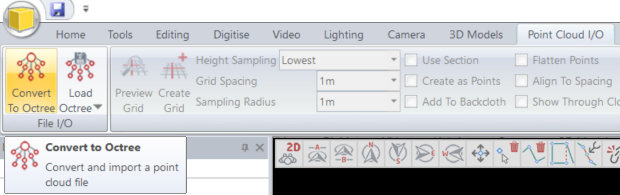
\includegraphics[width=1\linewidth]{obr4.png}
        \caption{Volba funkce pro převod mračna bodů do struktury Octree}
    \end{figure}
    \newpage
    \item V dialogovém okně klikneme na \textbf{Add Folder} a vybereme adresář obsahující surová data (zpravidla ve formátu .LAS nebo .LAZ).
    \newpage
    \begin{figure}[h]
        \centering
        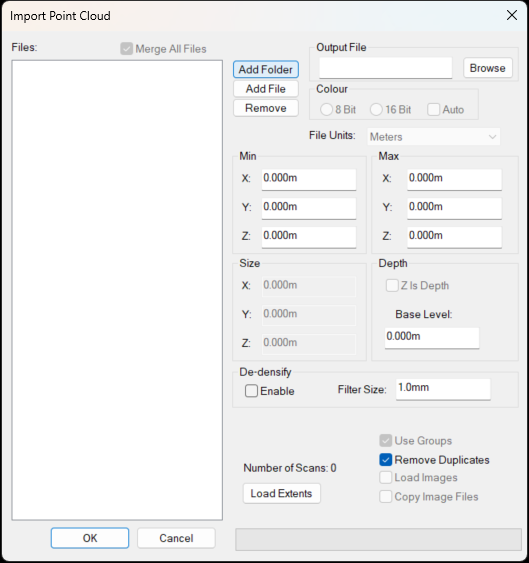
\includegraphics[width=1\linewidth]{obr5.png}
        \caption{Výběr adresáře se zdrojovými daty z mobilního skenování}
    \end{figure}
    
    \item Potvrdíme tlačítkem \textbf{OK}. Po dokončení konverze se mračno automaticky indexuje pro práci v prostředí N4CE.
\end{enumerate}
\subsection{Import panoramatických snímků}
Data z mobilního mapování jsou standardně rozdělena do dvou hlavních adresářů: \texttt{LAZ\_TILE} a \texttt{SPHERE}. Zatímco složka \texttt{LAZ\_TILE} obsahuje mračna bodů, v adresáři \texttt{SPHERE} jsou uloženy samotné panoramatické snímky a soubory nezbytné pro jejich korektní umístění a orientaci v prostoru.

Klíčovým prvkem jsou soubory s příponou \texttt{.csv}, které obsahují trajektorii vozidla, souřadnice středů snímků a jejich rotační parametry (roll, pitch, yaw). Bez těchto metadat nelze snímky s mračnem bodů přesně propojit.
\begin{figure}[h]
    \centering
    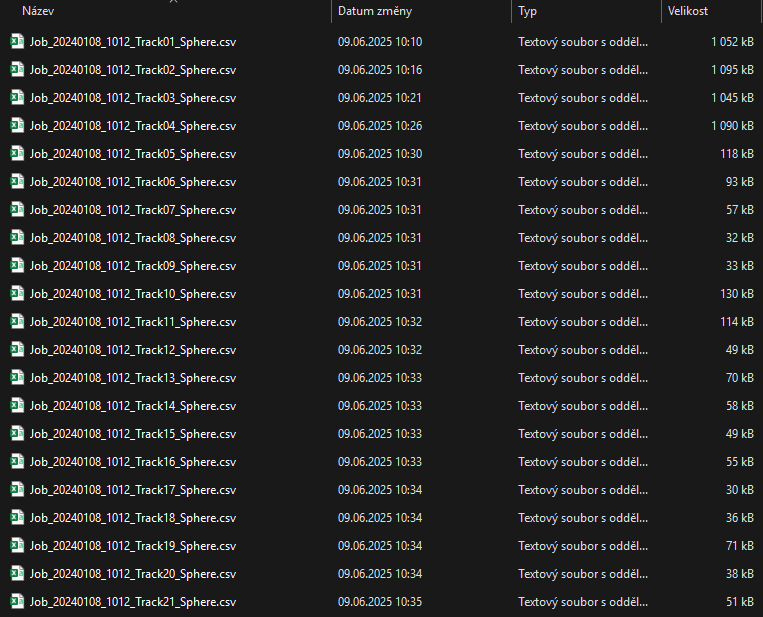
\includegraphics[width=1\linewidth]{obr6.png}
    \caption{Soubory metadat (.csv) pro orientaci panoramatických snímků}
\end{figure}

Při zkoumaní metadat ze složky \texttt{SPHERE} narážíme na specifický problém v kódování souřadnic S-JTSK. Soubory \texttt{.csv} sice obsahují korektní polohové údaje, avšak jsou zapsány s kladnými znaménky (absolutní hodnoty), což neodpovídá standardnímu geodetickému zápisu ve III. kvadrantu:
\begin{figure}[h]
    \centering
    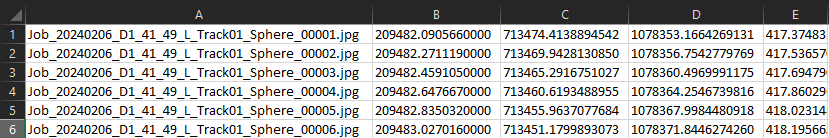
\includegraphics[width=1\linewidth]{obr7.png}
    \caption{Ukázka zdrojového .csv souboru – sloupce C a D obsahují kladné hodnoty souřadnic Y a X}
\end{figure}

Tato skutečnost způsobuje, že po importu by se panoramatické snímky zobrazily v jiném kvadrantu než mračna bodů. Dalším problémem je fakt, že \textbf{rotační parametry snímků} (úhly roll, pitch, yaw) jsou matematicky vázány na tento kladný souřadnicový systém. 

Pro správné sesazení snímků s mračnem proto nestačí pouhá změna znaménka u souřadnic. Je nezbytné provést simultánní transformaci polohy i rotací tak, aby orientace kamer odpovídala novému umístění v záporných hodnotách S-JTSK. K tomuto účelu využíváme skript v jazyce Python.
\subsubsection{Transformace dat Python skriptem}
Vzhledem k tomu, že ruční úprava desítek CSV souborů by byla časově neefektivní a náchylná k chybám, využíváme pro transformaci souřadnic a rotací následující \href{https://github.com/polucifier/n4ce-panorama-metadata-fix/blob/main/XY%20do%20-X-Y.py}{\textbf{skript v jazyce Python}}.
Následující kroky popisují, jak zprovoznit a spustit skript i v prostředí s omezenými uživatelskými právy.

\begin{enumerate}
    \item \textbf{Instalace Pythonu:} Pokud v systému není nainstalován interpret jazyka Python, nejsnadnější cestou je instalace z \textbf{Microsoft Store}. Tato verze nevyžaduje administrátorská oprávnění.
    \begin{figure}[h]
        \centering
        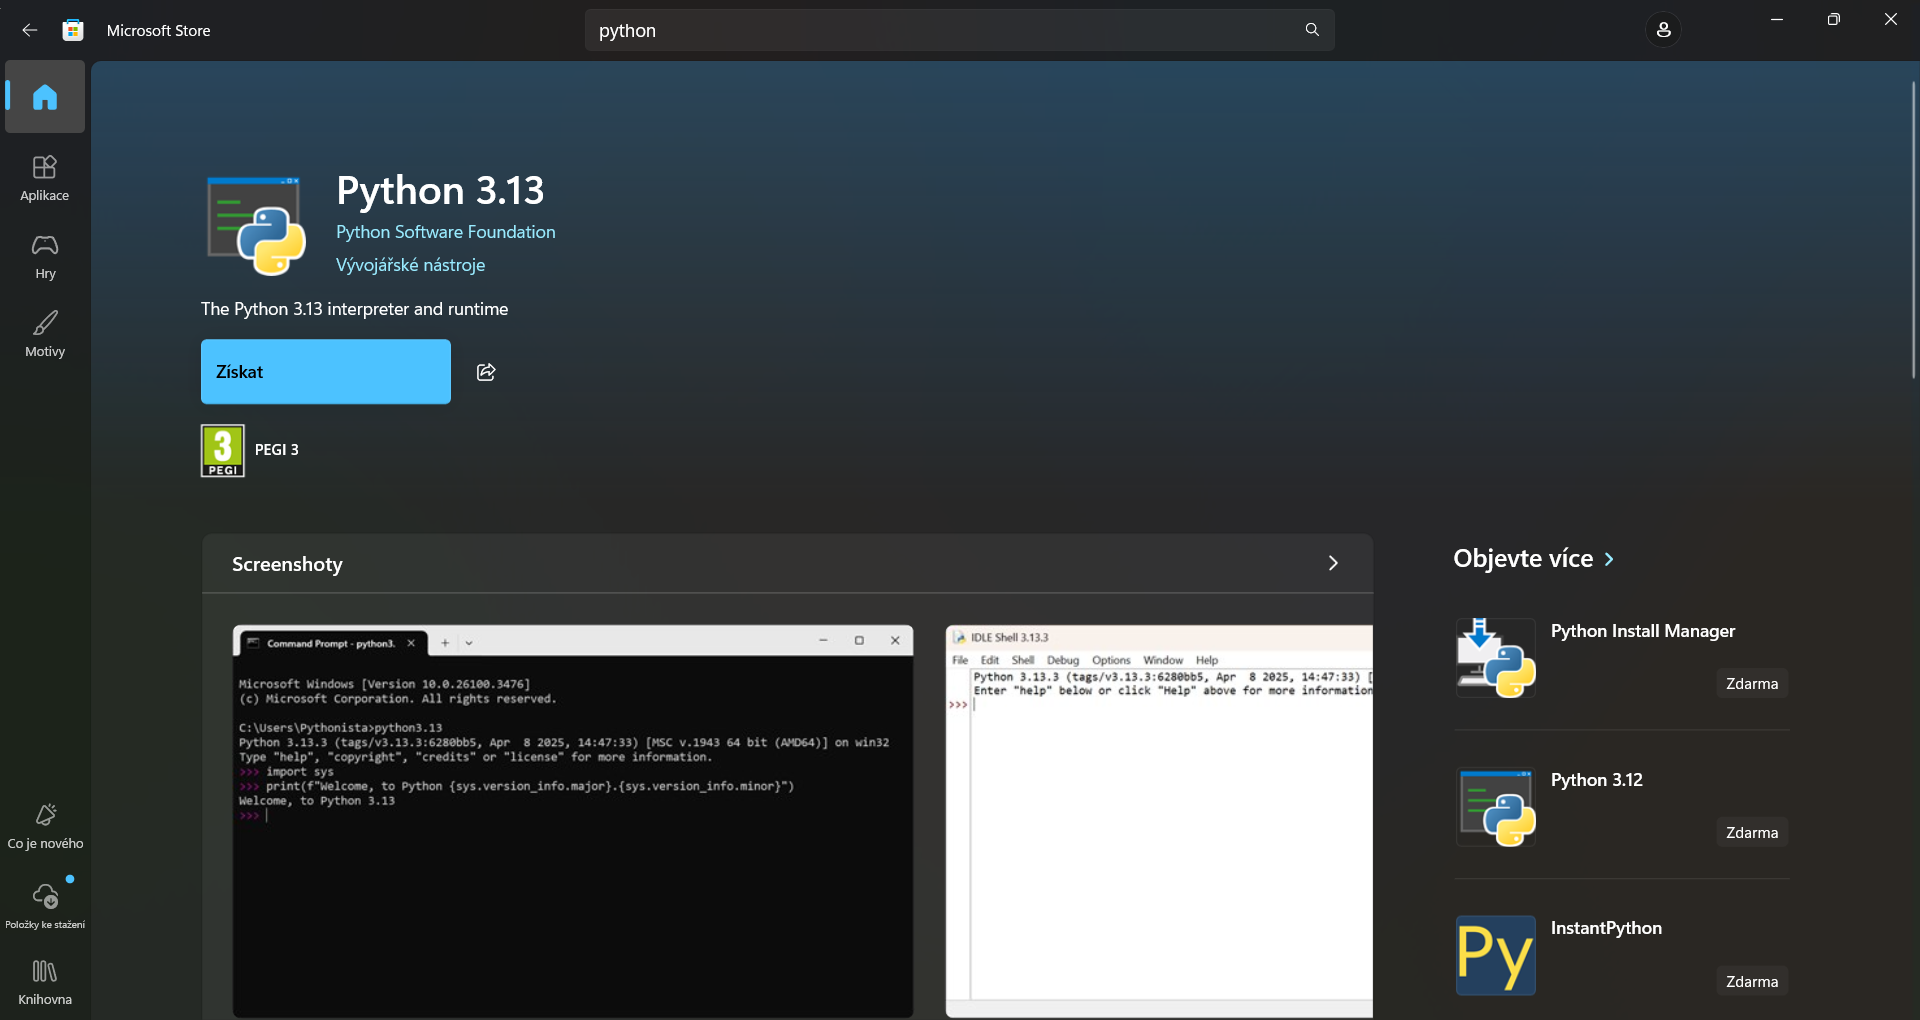
\includegraphics[width=1\linewidth]{obr8.png}
        \caption{Instalace Pythonu z Microsoft Store bez nutnosti práv správce}
    \end{figure}
    
    \item \textbf{Spuštění editoru IDLE:} Po instalaci vyhledáme v nabídce Start aplikaci \textbf{IDLE (Python GUI)} a spustíme ji. Jedná se o jednoduché vývojové prostředí, které je součástí standardní instalace.
    \begin{figure}[h]
        \centering
        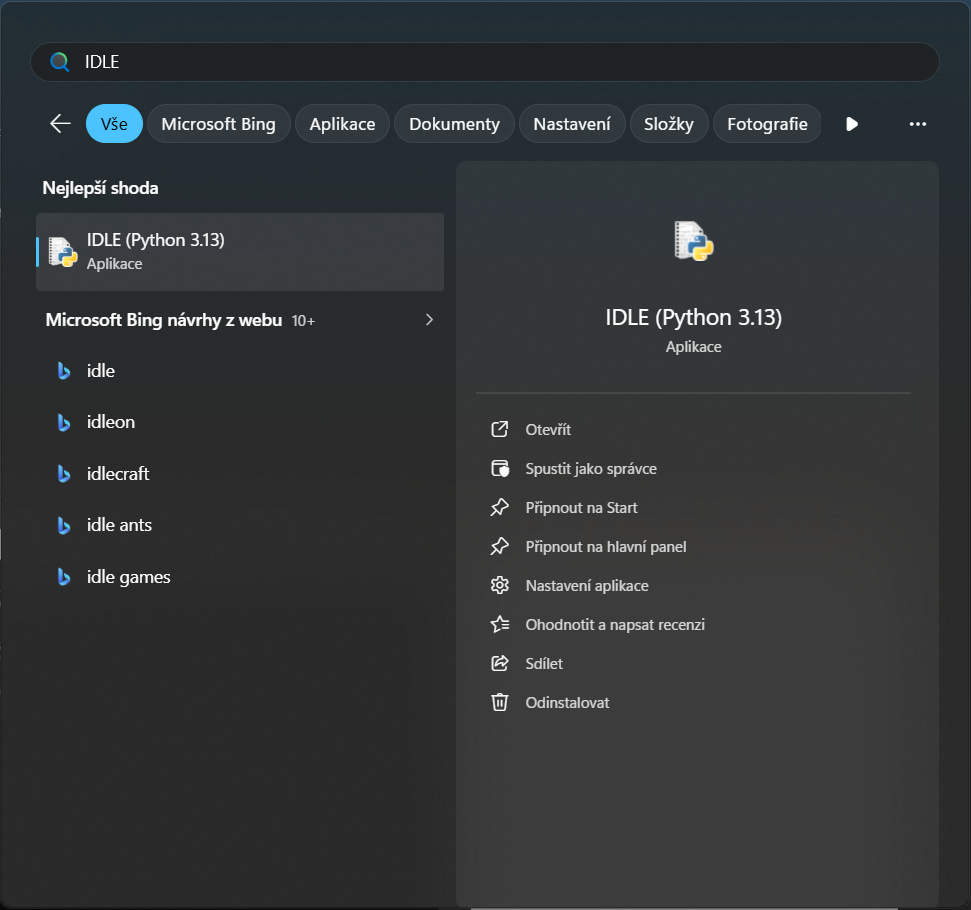
\includegraphics[width=1\linewidth]{obr9.png}
        \caption{Vyhledání a spuštění vývojového prostředí IDLE}
    \end{figure}
    \newpage
    \item \textbf{Příprava skriptu:} 
    \begin{itemize}
        \item Na GitHubu v repozitáři projektu zkopírujeme obsah skriptu pomocí tlačítka \textbf{Copy raw file}.
        \begin{figure}[h]
            \centering
            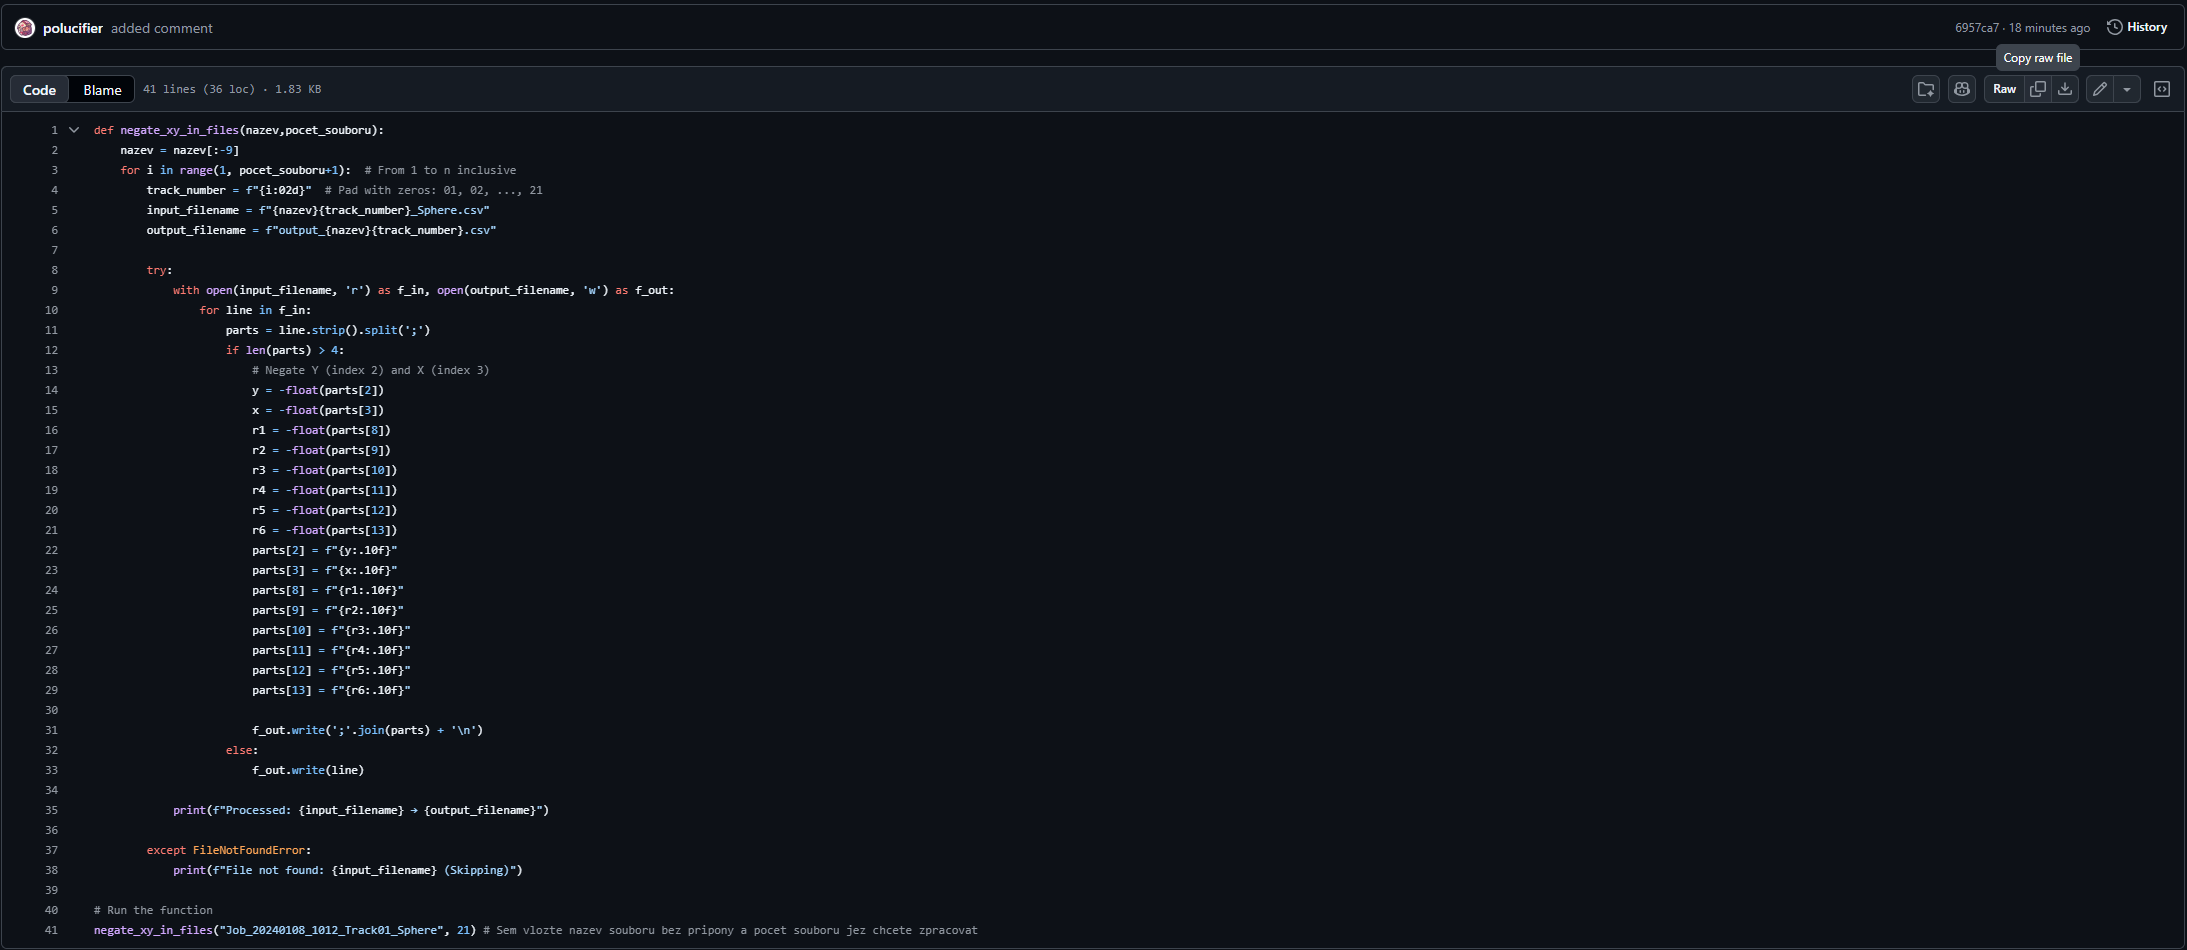
\includegraphics[width=1\linewidth]{obr10.png}
            \caption{Zkopírování zdrojového kódu z GitHubu}
        \end{figure}
        \newpage
        \item V editoru IDLE zvolíme \textit{File $\rightarrow$ New File}, vložíme zkopírovaný kód a soubor uložíme (např. jako \texttt{transformace.py}) do složky \texttt{SPHERE} k vašim datům.
    \end{itemize}
    \item \textbf{Konfigurace parametrů:} Před spuštěním je nutné na posledním řádku skriptu upravit textový řetězec tak, aby přesně odpovídal názvu vašich souborů, a zadat celkový počet tras ke zpracování.
    \begin{figure}[h]
        \centering
        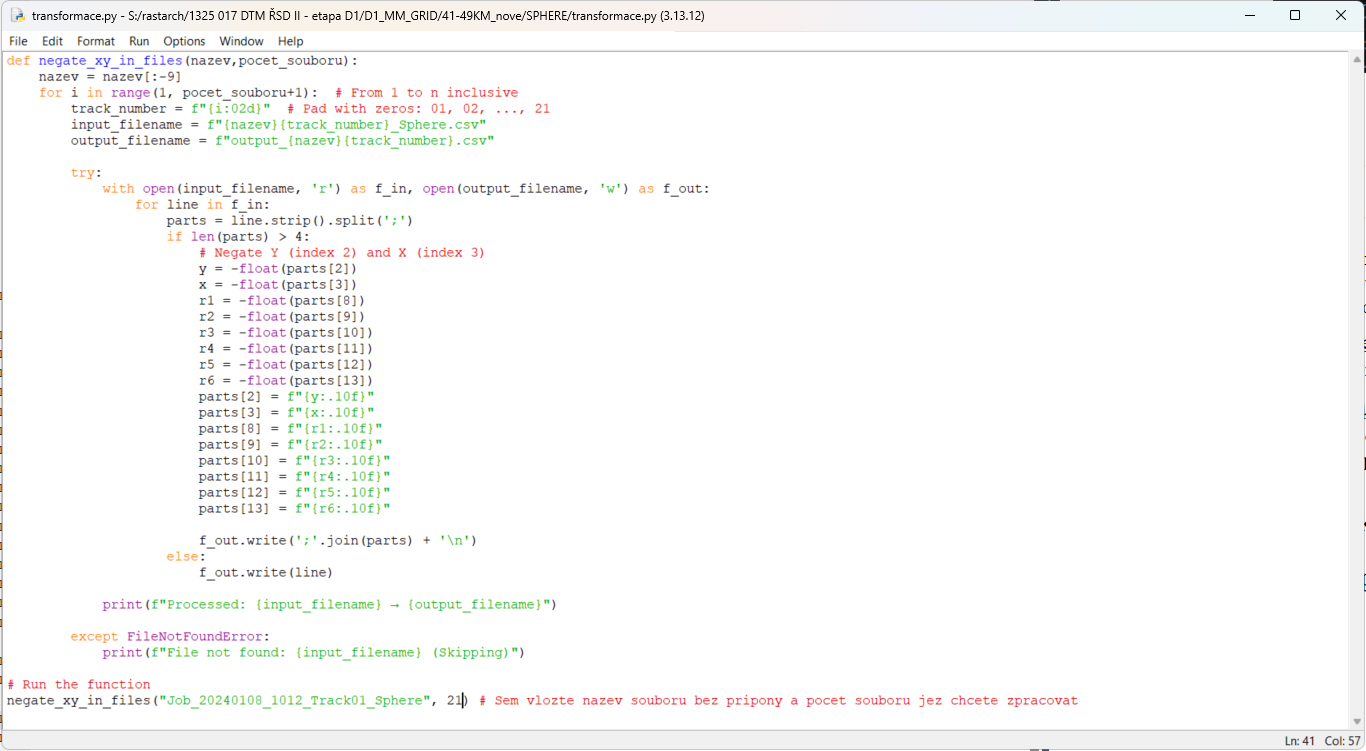
\includegraphics[width=1\linewidth]{obr11.png}
        \caption{Úprava názvu a počtu souborů před spuštěním}
    \end{figure}
    
    \item \textbf{Spuštění výpočtu:} Skript spustíme stisknutím klávesy \textbf{F5} nebo volbou v menu \textit{Run $\rightarrow$ Run Module}.
\end{enumerate}
Výsledkem operace jsou v cílovém adresáři vytvořené soubory s předponou \texttt{output}, které již mají korektní geodetickou polaritu a jsou připraveny pro bezchybný import do N4CE.
Jakmile máme připraveny transformované soubory metadat, můžeme přistoupit k jejich nahrání do projektu a vizualizaci pozic kamer přímo v mračnu bodů.

\begin{enumerate}
    \item \textbf{Aktivace importu:} V pracovním 3D okně přejdeme na záložku \textbf{Point Cloud Tools} a zvolíme funkci \textbf{Import $360^\circ$ Images}
    \begin{figure}[h]
    \centering
    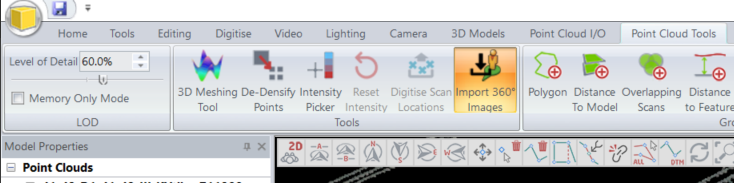
\includegraphics[width=1\linewidth]{obr12.png}
    \caption{Spuštění nástroje pro import panoramatických snímků}
    \end{figure}
    
    \item \textbf{Výběr zdroje:} V dialogovém okně, které se následně otevře, klikneme na tlačítko \textbf{Import Image}.
    \begin{figure}[h]
        \centering
        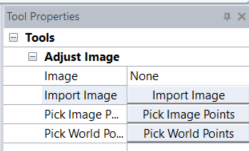
\includegraphics[width=0.5\linewidth]{obr13.png}
        \caption{Spuštění nástroje pro import panoramatických snímků}
    \end{figure}
    
    \item \textbf{Definice formátu:} Software N4CE vyžaduje specifikaci struktury vstupních dat. Pro naše upravené soubory zvolíme formát \textbf{Leica CSV}.
    \begin{figure}[h]
        \centering
        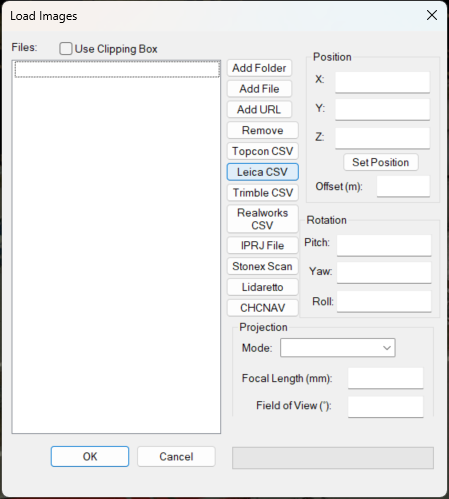
\includegraphics[width=0.9\linewidth]{obr14.png}
        \caption{Volba formátu Leica CSV pro import transformovaných metadat}
    \end{figure}
    \newpage
    
    \item \textbf{Hromadný výběr:} V prohlížeči souborů označíme všechny soubory s předponou \texttt{output}, které vygeneroval transformační skript, a potvrdíme tlačítkem \textbf{OK}.
    \begin{figure}[h]
        \centering
        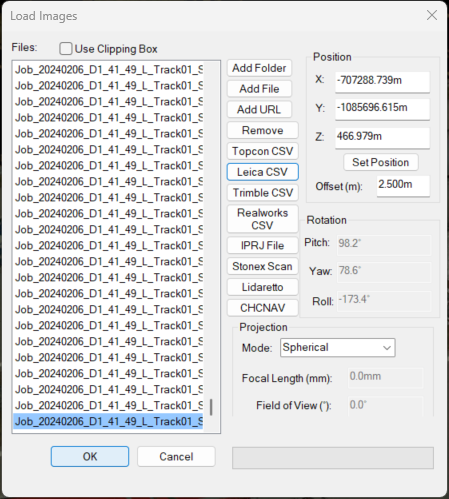
\includegraphics[width=0.9\linewidth]{obr15.png}
        \caption{Import panoramatických snímků}
    \end{figure}
    \newpage
    \item \textbf{Vizualizace v modelu:} Aby se pozice snímků v mračnu zobrazily, musíme v levém panelu \textbf{Model Properties} zaškrtnout volbu \textbf{Show Image Locations}.
    \begin{figure}[h]
        \centering
        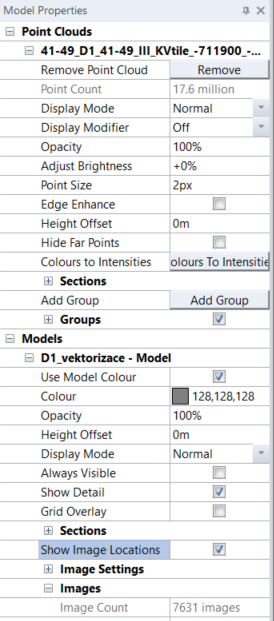
\includegraphics[width=0.4\linewidth]{obr16.png}
        \caption{Aktivace zobrazení pozic panoramatických snímků v panelu Model Properties}
    \end{figure}
\end{enumerate}
\newpage
Po úspěšném importu se v trase dálnice objeví symboly pozic jednotlivých snímků. Kliknutím levým tlačítkem myši na konkrétní symbol pozice se otevře okno \textbf{Image View}.
\begin{figure}[h]
    \centering
    \includegraphics[width=1\linewidth]{obr17.png}
    \caption{Symboly pozic jednotlivých snímků}
\end{figure}
\newpage

\section{Vektorizace prvků tělesa dálnice}
Vektorizaci lze provést v záložce \textbf{Digitise}.

\section{Export výsledků}
Po dokončení vektorizace všech prvků dálničního tělesa (hran vozovky, vodorovného značení, svodidel atd.) je možné data exportovat do formátu kompatibilního s CAD systémy.

V hlavním okně modelu přejdeme na záložku \textbf{Home}. Zde se nachází ikona pro export do AutoCADu. Klikneme na šipku pod tlačítkem \textbf{AutoCAD} a zvolíme možnost \textbf{Standard}.
\begin{figure}[h]
    \centering
    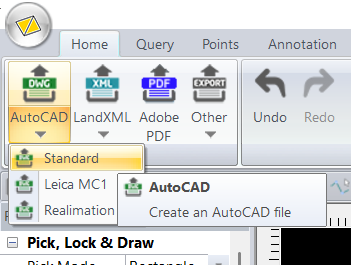
\includegraphics[width=0.5\linewidth]{Obr18.png}
    \caption{Výběr standardního typu exportu do formátu AutoCAD}
\end{figure}

\end{document}
